% Created by tikzDevice version 0.7.0 on 2014-09-22 20:38:32
% !TEX encoding = UTF-8 Unicode
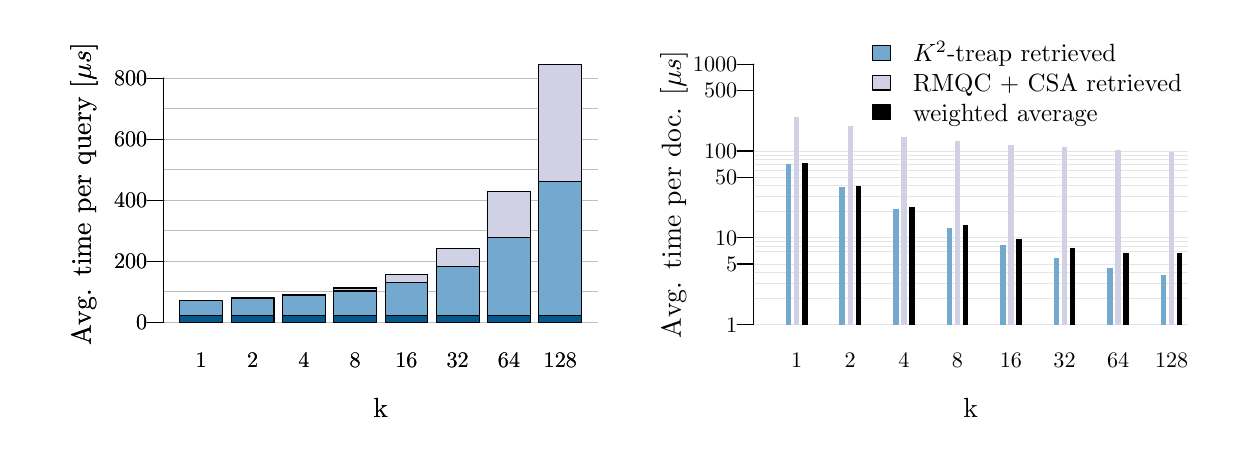
\begin{tikzpicture}[x=1pt,y=1pt]
\definecolor[named]{fillColor}{rgb}{1.00,1.00,1.00}
\path[use as bounding box,fill=fillColor,fill opacity=0.00] (0,0) rectangle (426.39,144.54);
\begin{scope}
\path[clip] (  0.00,  0.00) rectangle (213.20,144.54);
\definecolor[named]{drawColor}{rgb}{0.00,0.00,0.00}
\definecolor[named]{fillColor}{rgb}{0.02,0.35,0.55}

\path[draw=drawColor,line width= 0.4pt,line join=round,line cap=round,fill=fillColor] ( 55.01, 38.13) rectangle ( 70.45, 40.45);
\definecolor[named]{fillColor}{rgb}{0.45,0.66,0.81}

\path[draw=drawColor,line width= 0.4pt,line join=round,line cap=round,fill=fillColor] ( 55.01, 40.45) rectangle ( 70.45, 45.95);
\definecolor[named]{fillColor}{rgb}{0.82,0.82,0.90}

\path[draw=drawColor,line width= 0.4pt,line join=round,line cap=round,fill=fillColor] ( 55.01, 45.95) rectangle ( 70.45, 46.06);
\definecolor[named]{fillColor}{rgb}{0.02,0.35,0.55}

\path[draw=drawColor,line width= 0.4pt,line join=round,line cap=round,fill=fillColor] ( 73.54, 38.13) rectangle ( 88.99, 40.45);
\definecolor[named]{fillColor}{rgb}{0.45,0.66,0.81}

\path[draw=drawColor,line width= 0.4pt,line join=round,line cap=round,fill=fillColor] ( 73.54, 40.45) rectangle ( 88.99, 46.62);
\definecolor[named]{fillColor}{rgb}{0.82,0.82,0.90}

\path[draw=drawColor,line width= 0.4pt,line join=round,line cap=round,fill=fillColor] ( 73.54, 46.62) rectangle ( 88.99, 46.84);
\definecolor[named]{fillColor}{rgb}{0.02,0.35,0.55}

\path[draw=drawColor,line width= 0.4pt,line join=round,line cap=round,fill=fillColor] ( 92.08, 38.13) rectangle (107.52, 40.45);
\definecolor[named]{fillColor}{rgb}{0.45,0.66,0.81}

\path[draw=drawColor,line width= 0.4pt,line join=round,line cap=round,fill=fillColor] ( 92.08, 40.45) rectangle (107.52, 47.61);
\definecolor[named]{fillColor}{rgb}{0.82,0.82,0.90}

\path[draw=drawColor,line width= 0.4pt,line join=round,line cap=round,fill=fillColor] ( 92.08, 47.61) rectangle (107.52, 48.05);
\definecolor[named]{fillColor}{rgb}{0.02,0.35,0.55}

\path[draw=drawColor,line width= 0.4pt,line join=round,line cap=round,fill=fillColor] (110.61, 38.13) rectangle (126.05, 40.45);
\definecolor[named]{fillColor}{rgb}{0.45,0.66,0.81}

\path[draw=drawColor,line width= 0.4pt,line join=round,line cap=round,fill=fillColor] (110.61, 40.45) rectangle (126.05, 49.37);
\definecolor[named]{fillColor}{rgb}{0.82,0.82,0.90}

\path[draw=drawColor,line width= 0.4pt,line join=round,line cap=round,fill=fillColor] (110.61, 49.37) rectangle (126.05, 50.47);
\definecolor[named]{fillColor}{rgb}{0.02,0.35,0.55}

\path[draw=drawColor,line width= 0.4pt,line join=round,line cap=round,fill=fillColor] (129.14, 38.13) rectangle (144.59, 40.45);
\definecolor[named]{fillColor}{rgb}{0.45,0.66,0.81}

\path[draw=drawColor,line width= 0.4pt,line join=round,line cap=round,fill=fillColor] (129.14, 40.45) rectangle (144.59, 52.56);
\definecolor[named]{fillColor}{rgb}{0.82,0.82,0.90}

\path[draw=drawColor,line width= 0.4pt,line join=round,line cap=round,fill=fillColor] (129.14, 52.56) rectangle (144.59, 55.21);
\definecolor[named]{fillColor}{rgb}{0.02,0.35,0.55}

\path[draw=drawColor,line width= 0.4pt,line join=round,line cap=round,fill=fillColor] (147.68, 38.13) rectangle (163.12, 40.45);
\definecolor[named]{fillColor}{rgb}{0.45,0.66,0.81}

\path[draw=drawColor,line width= 0.4pt,line join=round,line cap=round,fill=fillColor] (147.68, 40.45) rectangle (163.12, 58.29);
\definecolor[named]{fillColor}{rgb}{0.82,0.82,0.90}

\path[draw=drawColor,line width= 0.4pt,line join=round,line cap=round,fill=fillColor] (147.68, 58.29) rectangle (163.12, 64.90);
\definecolor[named]{fillColor}{rgb}{0.02,0.35,0.55}

\path[draw=drawColor,line width= 0.4pt,line join=round,line cap=round,fill=fillColor] (166.21, 38.13) rectangle (181.66, 40.45);
\definecolor[named]{fillColor}{rgb}{0.45,0.66,0.81}

\path[draw=drawColor,line width= 0.4pt,line join=round,line cap=round,fill=fillColor] (166.21, 40.45) rectangle (181.66, 68.65);
\definecolor[named]{fillColor}{rgb}{0.82,0.82,0.90}

\path[draw=drawColor,line width= 0.4pt,line join=round,line cap=round,fill=fillColor] (166.21, 68.65) rectangle (181.66, 85.40);
\definecolor[named]{fillColor}{rgb}{0.02,0.35,0.55}

\path[draw=drawColor,line width= 0.4pt,line join=round,line cap=round,fill=fillColor] (184.74, 38.13) rectangle (200.19, 40.45);
\definecolor[named]{fillColor}{rgb}{0.45,0.66,0.81}

\path[draw=drawColor,line width= 0.4pt,line join=round,line cap=round,fill=fillColor] (184.74, 40.45) rectangle (200.19, 88.81);
\definecolor[named]{fillColor}{rgb}{0.82,0.82,0.90}

\path[draw=drawColor,line width= 0.4pt,line join=round,line cap=round,fill=fillColor] (184.74, 88.81) rectangle (200.19,131.34);
\end{scope}
\begin{scope}
\path[clip] (  0.00,  0.00) rectangle (426.39,144.54);
\definecolor[named]{drawColor}{rgb}{0.00,0.00,0.00}

\node[text=drawColor,anchor=base,inner sep=0pt, outer sep=0pt, scale=  0.80] at ( 62.73, 21.60) {1};

\node[text=drawColor,anchor=base,inner sep=0pt, outer sep=0pt, scale=  0.80] at ( 81.26, 21.60) {2};

\node[text=drawColor,anchor=base,inner sep=0pt, outer sep=0pt, scale=  0.80] at ( 99.80, 21.60) {4};

\node[text=drawColor,anchor=base,inner sep=0pt, outer sep=0pt, scale=  0.80] at (118.33, 21.60) {8};

\node[text=drawColor,anchor=base,inner sep=0pt, outer sep=0pt, scale=  0.80] at (136.87, 21.60) {16};

\node[text=drawColor,anchor=base,inner sep=0pt, outer sep=0pt, scale=  0.80] at (155.40, 21.60) {32};

\node[text=drawColor,anchor=base,inner sep=0pt, outer sep=0pt, scale=  0.80] at (173.93, 21.60) {64};

\node[text=drawColor,anchor=base,inner sep=0pt, outer sep=0pt, scale=  0.80] at (192.47, 21.60) {128};
\end{scope}
\begin{scope}
\path[clip] (  0.00,  0.00) rectangle (213.20,144.54);
\definecolor[named]{drawColor}{rgb}{0.00,0.00,0.00}

\node[text=drawColor,anchor=base,inner sep=0pt, outer sep=0pt, scale=  1.00] at (127.60,  3.60) {k};

\node[text=drawColor,rotate= 90.00,anchor=base,inner sep=0pt, outer sep=0pt, scale=  1.00] at ( 22.80, 84.27) {Avg. time per query [$\mu s$]};
\end{scope}
\begin{scope}
\path[clip] (  0.00,  0.00) rectangle (426.39,144.54);
\definecolor[named]{drawColor}{rgb}{0.00,0.00,0.00}

\path[draw=drawColor,line width= 0.4pt,line join=round,line cap=round] ( 49.20, 38.13) -- ( 49.20,126.27);

\path[draw=drawColor,line width= 0.4pt,line join=round,line cap=round] ( 49.20, 38.13) -- ( 43.20, 38.13);

\path[draw=drawColor,line width= 0.4pt,line join=round,line cap=round] ( 49.20, 60.17) -- ( 43.20, 60.17);

\path[draw=drawColor,line width= 0.4pt,line join=round,line cap=round] ( 49.20, 82.20) -- ( 43.20, 82.20);

\path[draw=drawColor,line width= 0.4pt,line join=round,line cap=round] ( 49.20,104.24) -- ( 43.20,104.24);

\path[draw=drawColor,line width= 0.4pt,line join=round,line cap=round] ( 49.20,126.27) -- ( 43.20,126.27);

\node[text=drawColor,anchor=base east,inner sep=0pt, outer sep=0pt, scale=  0.80] at ( 43.20, 35.38) {0};

\node[text=drawColor,anchor=base east,inner sep=0pt, outer sep=0pt, scale=  0.80] at ( 43.20, 57.41) {200};

\node[text=drawColor,anchor=base east,inner sep=0pt, outer sep=0pt, scale=  0.80] at ( 43.20, 79.45) {400};

\node[text=drawColor,anchor=base east,inner sep=0pt, outer sep=0pt, scale=  0.80] at ( 43.20,101.48) {600};

\node[text=drawColor,anchor=base east,inner sep=0pt, outer sep=0pt, scale=  0.80] at ( 43.20,123.52) {800};
\end{scope}
\begin{scope}
\path[clip] ( 49.20, 37.20) rectangle (206.00,131.34);
\definecolor[named]{drawColor}{rgb}{0.75,0.75,0.75}

\path[draw=drawColor,line width= 0.4pt,line join=round,line cap=round] ( 49.20, 38.13) -- (206.00, 38.13);

\path[draw=drawColor,line width= 0.4pt,line join=round,line cap=round] ( 49.20, 49.15) -- (206.00, 49.15);

\path[draw=drawColor,line width= 0.4pt,line join=round,line cap=round] ( 49.20, 60.17) -- (206.00, 60.17);

\path[draw=drawColor,line width= 0.4pt,line join=round,line cap=round] ( 49.20, 71.18) -- (206.00, 71.18);

\path[draw=drawColor,line width= 0.4pt,line join=round,line cap=round] ( 49.20, 82.20) -- (206.00, 82.20);

\path[draw=drawColor,line width= 0.4pt,line join=round,line cap=round] ( 49.20, 93.22) -- (206.00, 93.22);

\path[draw=drawColor,line width= 0.4pt,line join=round,line cap=round] ( 49.20,104.24) -- (206.00,104.24);

\path[draw=drawColor,line width= 0.4pt,line join=round,line cap=round] ( 49.20,115.25) -- (206.00,115.25);

\path[draw=drawColor,line width= 0.4pt,line join=round,line cap=round] ( 49.20,126.27) -- (206.00,126.27);
\end{scope}
\begin{scope}
\path[clip] (  0.00,  0.00) rectangle (213.20,144.54);
\definecolor[named]{drawColor}{rgb}{0.00,0.00,0.00}
\definecolor[named]{fillColor}{rgb}{0.02,0.35,0.55}

\path[draw=drawColor,line width= 0.4pt,line join=round,line cap=round,fill=fillColor] ( 55.01, 38.13) rectangle ( 70.45, 40.45);
\definecolor[named]{fillColor}{rgb}{0.45,0.66,0.81}

\path[draw=drawColor,line width= 0.4pt,line join=round,line cap=round,fill=fillColor] ( 55.01, 40.45) rectangle ( 70.45, 45.95);
\definecolor[named]{fillColor}{rgb}{0.82,0.82,0.90}

\path[draw=drawColor,line width= 0.4pt,line join=round,line cap=round,fill=fillColor] ( 55.01, 45.95) rectangle ( 70.45, 46.06);
\definecolor[named]{fillColor}{rgb}{0.02,0.35,0.55}

\path[draw=drawColor,line width= 0.4pt,line join=round,line cap=round,fill=fillColor] ( 73.54, 38.13) rectangle ( 88.99, 40.45);
\definecolor[named]{fillColor}{rgb}{0.45,0.66,0.81}

\path[draw=drawColor,line width= 0.4pt,line join=round,line cap=round,fill=fillColor] ( 73.54, 40.45) rectangle ( 88.99, 46.62);
\definecolor[named]{fillColor}{rgb}{0.82,0.82,0.90}

\path[draw=drawColor,line width= 0.4pt,line join=round,line cap=round,fill=fillColor] ( 73.54, 46.62) rectangle ( 88.99, 46.84);
\definecolor[named]{fillColor}{rgb}{0.02,0.35,0.55}

\path[draw=drawColor,line width= 0.4pt,line join=round,line cap=round,fill=fillColor] ( 92.08, 38.13) rectangle (107.52, 40.45);
\definecolor[named]{fillColor}{rgb}{0.45,0.66,0.81}

\path[draw=drawColor,line width= 0.4pt,line join=round,line cap=round,fill=fillColor] ( 92.08, 40.45) rectangle (107.52, 47.61);
\definecolor[named]{fillColor}{rgb}{0.82,0.82,0.90}

\path[draw=drawColor,line width= 0.4pt,line join=round,line cap=round,fill=fillColor] ( 92.08, 47.61) rectangle (107.52, 48.05);
\definecolor[named]{fillColor}{rgb}{0.02,0.35,0.55}

\path[draw=drawColor,line width= 0.4pt,line join=round,line cap=round,fill=fillColor] (110.61, 38.13) rectangle (126.05, 40.45);
\definecolor[named]{fillColor}{rgb}{0.45,0.66,0.81}

\path[draw=drawColor,line width= 0.4pt,line join=round,line cap=round,fill=fillColor] (110.61, 40.45) rectangle (126.05, 49.37);
\definecolor[named]{fillColor}{rgb}{0.82,0.82,0.90}

\path[draw=drawColor,line width= 0.4pt,line join=round,line cap=round,fill=fillColor] (110.61, 49.37) rectangle (126.05, 50.47);
\definecolor[named]{fillColor}{rgb}{0.02,0.35,0.55}

\path[draw=drawColor,line width= 0.4pt,line join=round,line cap=round,fill=fillColor] (129.14, 38.13) rectangle (144.59, 40.45);
\definecolor[named]{fillColor}{rgb}{0.45,0.66,0.81}

\path[draw=drawColor,line width= 0.4pt,line join=round,line cap=round,fill=fillColor] (129.14, 40.45) rectangle (144.59, 52.56);
\definecolor[named]{fillColor}{rgb}{0.82,0.82,0.90}

\path[draw=drawColor,line width= 0.4pt,line join=round,line cap=round,fill=fillColor] (129.14, 52.56) rectangle (144.59, 55.21);
\definecolor[named]{fillColor}{rgb}{0.02,0.35,0.55}

\path[draw=drawColor,line width= 0.4pt,line join=round,line cap=round,fill=fillColor] (147.68, 38.13) rectangle (163.12, 40.45);
\definecolor[named]{fillColor}{rgb}{0.45,0.66,0.81}

\path[draw=drawColor,line width= 0.4pt,line join=round,line cap=round,fill=fillColor] (147.68, 40.45) rectangle (163.12, 58.29);
\definecolor[named]{fillColor}{rgb}{0.82,0.82,0.90}

\path[draw=drawColor,line width= 0.4pt,line join=round,line cap=round,fill=fillColor] (147.68, 58.29) rectangle (163.12, 64.90);
\definecolor[named]{fillColor}{rgb}{0.02,0.35,0.55}

\path[draw=drawColor,line width= 0.4pt,line join=round,line cap=round,fill=fillColor] (166.21, 38.13) rectangle (181.66, 40.45);
\definecolor[named]{fillColor}{rgb}{0.45,0.66,0.81}

\path[draw=drawColor,line width= 0.4pt,line join=round,line cap=round,fill=fillColor] (166.21, 40.45) rectangle (181.66, 68.65);
\definecolor[named]{fillColor}{rgb}{0.82,0.82,0.90}

\path[draw=drawColor,line width= 0.4pt,line join=round,line cap=round,fill=fillColor] (166.21, 68.65) rectangle (181.66, 85.40);
\definecolor[named]{fillColor}{rgb}{0.02,0.35,0.55}

\path[draw=drawColor,line width= 0.4pt,line join=round,line cap=round,fill=fillColor] (184.74, 38.13) rectangle (200.19, 40.45);
\definecolor[named]{fillColor}{rgb}{0.45,0.66,0.81}

\path[draw=drawColor,line width= 0.4pt,line join=round,line cap=round,fill=fillColor] (184.74, 40.45) rectangle (200.19, 88.81);
\definecolor[named]{fillColor}{rgb}{0.82,0.82,0.90}

\path[draw=drawColor,line width= 0.4pt,line join=round,line cap=round,fill=fillColor] (184.74, 88.81) rectangle (200.19,131.34);
\end{scope}
\begin{scope}
\path[clip] (  0.00,  0.00) rectangle (426.39,144.54);
\definecolor[named]{drawColor}{rgb}{0.00,0.00,0.00}

\node[text=drawColor,anchor=base,inner sep=0pt, outer sep=0pt, scale=  0.80] at ( 62.73, 21.60) {1};

\node[text=drawColor,anchor=base,inner sep=0pt, outer sep=0pt, scale=  0.80] at ( 81.26, 21.60) {2};

\node[text=drawColor,anchor=base,inner sep=0pt, outer sep=0pt, scale=  0.80] at ( 99.80, 21.60) {4};

\node[text=drawColor,anchor=base,inner sep=0pt, outer sep=0pt, scale=  0.80] at (118.33, 21.60) {8};

\node[text=drawColor,anchor=base,inner sep=0pt, outer sep=0pt, scale=  0.80] at (136.87, 21.60) {16};

\node[text=drawColor,anchor=base,inner sep=0pt, outer sep=0pt, scale=  0.80] at (155.40, 21.60) {32};

\node[text=drawColor,anchor=base,inner sep=0pt, outer sep=0pt, scale=  0.80] at (173.93, 21.60) {64};

\node[text=drawColor,anchor=base,inner sep=0pt, outer sep=0pt, scale=  0.80] at (192.47, 21.60) {128};
\end{scope}
\begin{scope}
\path[clip] (  0.00,  0.00) rectangle (213.20,144.54);
\definecolor[named]{drawColor}{rgb}{0.00,0.00,0.00}

\node[text=drawColor,anchor=base,inner sep=0pt, outer sep=0pt, scale=  1.00] at (127.60,  3.60) {k};

\node[text=drawColor,rotate= 90.00,anchor=base,inner sep=0pt, outer sep=0pt, scale=  1.00] at ( 22.80, 84.27) {Avg. time per query [$\mu s$]};
\end{scope}
\begin{scope}
\path[clip] (  0.00,  0.00) rectangle (426.39,144.54);
\definecolor[named]{drawColor}{rgb}{0.00,0.00,0.00}

\path[draw=drawColor,line width= 0.4pt,line join=round,line cap=round] ( 49.20, 38.13) -- ( 49.20,126.27);

\path[draw=drawColor,line width= 0.4pt,line join=round,line cap=round] ( 49.20, 38.13) -- ( 43.20, 38.13);

\path[draw=drawColor,line width= 0.4pt,line join=round,line cap=round] ( 49.20, 60.17) -- ( 43.20, 60.17);

\path[draw=drawColor,line width= 0.4pt,line join=round,line cap=round] ( 49.20, 82.20) -- ( 43.20, 82.20);

\path[draw=drawColor,line width= 0.4pt,line join=round,line cap=round] ( 49.20,104.24) -- ( 43.20,104.24);

\path[draw=drawColor,line width= 0.4pt,line join=round,line cap=round] ( 49.20,126.27) -- ( 43.20,126.27);

\node[text=drawColor,anchor=base east,inner sep=0pt, outer sep=0pt, scale=  0.80] at ( 43.20, 35.38) {0};

\node[text=drawColor,anchor=base east,inner sep=0pt, outer sep=0pt, scale=  0.80] at ( 43.20, 57.41) {200};

\node[text=drawColor,anchor=base east,inner sep=0pt, outer sep=0pt, scale=  0.80] at ( 43.20, 79.45) {400};

\node[text=drawColor,anchor=base east,inner sep=0pt, outer sep=0pt, scale=  0.80] at ( 43.20,101.48) {600};

\node[text=drawColor,anchor=base east,inner sep=0pt, outer sep=0pt, scale=  0.80] at ( 43.20,123.52) {800};
\end{scope}
\begin{scope}
\path[clip] (  0.00,  0.00) rectangle (426.39,144.54);
\definecolor[named]{drawColor}{rgb}{0.00,0.00,0.00}

\path[draw=drawColor,line width= 0.4pt,line join=round,line cap=round] (262.40, 37.20) -- (262.40,131.34);

\path[draw=drawColor,line width= 0.4pt,line join=round,line cap=round] (262.40, 37.20) -- (256.40, 37.20);

\path[draw=drawColor,line width= 0.4pt,line join=round,line cap=round] (262.40, 59.13) -- (256.40, 59.13);

\path[draw=drawColor,line width= 0.4pt,line join=round,line cap=round] (262.40, 68.58) -- (256.40, 68.58);

\path[draw=drawColor,line width= 0.4pt,line join=round,line cap=round] (262.40, 90.51) -- (256.40, 90.51);

\path[draw=drawColor,line width= 0.4pt,line join=round,line cap=round] (262.40, 99.96) -- (256.40, 99.96);

\path[draw=drawColor,line width= 0.4pt,line join=round,line cap=round] (262.40,121.89) -- (256.40,121.89);

\path[draw=drawColor,line width= 0.4pt,line join=round,line cap=round] (262.40,131.34) -- (256.40,131.34);

\node[text=drawColor,anchor=base east,inner sep=0pt, outer sep=0pt, scale=  0.80] at (256.40, 34.45) {1};

\node[text=drawColor,anchor=base east,inner sep=0pt, outer sep=0pt, scale=  0.80] at (256.40, 56.38) {5};

\node[text=drawColor,anchor=base east,inner sep=0pt, outer sep=0pt, scale=  0.80] at (256.40, 65.83) {10};

\node[text=drawColor,anchor=base east,inner sep=0pt, outer sep=0pt, scale=  0.80] at (256.40, 87.76) {50};

\node[text=drawColor,anchor=base east,inner sep=0pt, outer sep=0pt, scale=  0.80] at (256.40, 97.21) {100};

\node[text=drawColor,anchor=base east,inner sep=0pt, outer sep=0pt, scale=  0.80] at (256.40,119.14) {500};

\node[text=drawColor,anchor=base east,inner sep=0pt, outer sep=0pt, scale=  0.80] at (256.40,128.59) {1000};
\end{scope}
\begin{scope}
\path[clip] (213.20,  0.00) rectangle (426.39,144.54);
\definecolor[named]{drawColor}{rgb}{0.00,0.00,0.00}

\node[text=drawColor,anchor=base,inner sep=0pt, outer sep=0pt, scale=  1.00] at (340.79,  3.60) {k};

\node[text=drawColor,rotate= 90.00,anchor=base,inner sep=0pt, outer sep=0pt, scale=  1.00] at (236.00, 84.27) {Avg. time per doc. [$\mu s$]};
\end{scope}
\begin{scope}
\path[clip] (262.40, 37.20) rectangle (419.19,131.34);
\definecolor[named]{drawColor}{rgb}{0.90,0.90,0.90}

\path[draw=drawColor,line width= 0.3pt,line join=round,line cap=round] (262.40, 37.20) -- (419.19, 37.20);

\path[draw=drawColor,line width= 0.3pt,line join=round,line cap=round] (262.40, 46.65) -- (419.19, 46.65);

\path[draw=drawColor,line width= 0.3pt,line join=round,line cap=round] (262.40, 52.17) -- (419.19, 52.17);

\path[draw=drawColor,line width= 0.3pt,line join=round,line cap=round] (262.40, 56.09) -- (419.19, 56.09);

\path[draw=drawColor,line width= 0.3pt,line join=round,line cap=round] (262.40, 59.13) -- (419.19, 59.13);

\path[draw=drawColor,line width= 0.3pt,line join=round,line cap=round] (262.40, 65.54) -- (419.19, 65.54);

\path[draw=drawColor,line width= 0.3pt,line join=round,line cap=round] (262.40, 63.72) -- (419.19, 63.72);

\path[draw=drawColor,line width= 0.3pt,line join=round,line cap=round] (262.40, 65.54) -- (419.19, 65.54);

\path[draw=drawColor,line width= 0.3pt,line join=round,line cap=round] (262.40, 67.14) -- (419.19, 67.14);

\path[draw=drawColor,line width= 0.3pt,line join=round,line cap=round] (262.40, 68.58) -- (419.19, 68.58);

\path[draw=drawColor,line width= 0.3pt,line join=round,line cap=round] (262.40, 78.03) -- (419.19, 78.03);

\path[draw=drawColor,line width= 0.3pt,line join=round,line cap=round] (262.40, 83.55) -- (419.19, 83.55);

\path[draw=drawColor,line width= 0.3pt,line join=round,line cap=round] (262.40, 87.47) -- (419.19, 87.47);

\path[draw=drawColor,line width= 0.3pt,line join=round,line cap=round] (262.40, 90.51) -- (419.19, 90.51);

\path[draw=drawColor,line width= 0.3pt,line join=round,line cap=round] (262.40, 93.00) -- (419.19, 93.00);

\path[draw=drawColor,line width= 0.3pt,line join=round,line cap=round] (262.40, 95.10) -- (419.19, 95.10);

\path[draw=drawColor,line width= 0.3pt,line join=round,line cap=round] (262.40, 96.92) -- (419.19, 96.92);

\path[draw=drawColor,line width= 0.3pt,line join=round,line cap=round] (262.40, 98.52) -- (419.19, 98.52);

\path[draw=drawColor,line width= 0.3pt,line join=round,line cap=round] (262.40, 99.96) -- (419.19, 99.96);
\end{scope}
\begin{scope}
\path[clip] (  0.00,  0.00) rectangle (426.39,144.54);
\definecolor[named]{drawColor}{rgb}{0.00,0.00,0.00}

\node[text=drawColor,anchor=base,inner sep=0pt, outer sep=0pt, scale=  0.80] at (277.88, 21.60) {1};

\node[text=drawColor,anchor=base,inner sep=0pt, outer sep=0pt, scale=  0.80] at (297.24, 21.60) {2};

\node[text=drawColor,anchor=base,inner sep=0pt, outer sep=0pt, scale=  0.80] at (316.60, 21.60) {4};

\node[text=drawColor,anchor=base,inner sep=0pt, outer sep=0pt, scale=  0.80] at (335.96, 21.60) {8};

\node[text=drawColor,anchor=base,inner sep=0pt, outer sep=0pt, scale=  0.80] at (355.31, 21.60) {16};

\node[text=drawColor,anchor=base,inner sep=0pt, outer sep=0pt, scale=  0.80] at (374.67, 21.60) {32};

\node[text=drawColor,anchor=base,inner sep=0pt, outer sep=0pt, scale=  0.80] at (394.03, 21.60) {64};

\node[text=drawColor,anchor=base,inner sep=0pt, outer sep=0pt, scale=  0.80] at (413.39, 21.60) {128};
\end{scope}
\begin{scope}
\path[clip] (213.20,  0.00) rectangle (426.39,144.54);
\definecolor[named]{drawColor}{rgb}{0.00,0.00,0.00}
\definecolor[named]{fillColor}{rgb}{0.45,0.66,0.81}

\path[draw=drawColor,line width= 0.4pt,line join=round,line cap=round,fill=fillColor] (305.34,138.21) rectangle (311.82,132.81);
\definecolor[named]{fillColor}{rgb}{0.82,0.82,0.90}

\path[draw=drawColor,line width= 0.4pt,line join=round,line cap=round,fill=fillColor] (305.34,127.41) rectangle (311.82,122.01);
\definecolor[named]{fillColor}{rgb}{0.00,0.00,0.00}

\path[draw=drawColor,line width= 0.4pt,line join=round,line cap=round,fill=fillColor] (305.34,116.61) rectangle (311.82,111.21);

\node[text=drawColor,anchor=base west,inner sep=0pt, outer sep=0pt, scale=  0.90] at (319.92,132.41) {$K^2$-treap retrieved};

\node[text=drawColor,anchor=base west,inner sep=0pt, outer sep=0pt, scale=  0.90] at (319.92,121.61) {RMQC + CSA retrieved};

\node[text=drawColor,anchor=base west,inner sep=0pt, outer sep=0pt, scale=  0.90] at (319.92,110.81) {weighted average};
\end{scope}
\begin{scope}
\path[clip] (262.40, 37.20) rectangle (419.19,131.34);
\definecolor[named]{drawColor}{rgb}{0.45,0.66,0.81}

\path[draw=drawColor,line width= 2.0pt,line join=round] (274.98, 37.20) --
	(274.98, 95.35);
\definecolor[named]{drawColor}{rgb}{0.00,0.00,0.00}

\path[draw=drawColor,line width= 2.0pt,line join=round] (280.79, 37.20) --
	(280.79, 95.48);
\definecolor[named]{drawColor}{rgb}{0.82,0.82,0.90}

\path[draw=drawColor,line width= 2.0pt,line join=round] (277.88, 37.20) --
	(277.88,112.28);
\definecolor[named]{drawColor}{rgb}{0.45,0.66,0.81}

\path[draw=drawColor,line width= 2.0pt,line join=round] (294.34, 37.20) --
	(294.34, 87.03);
\definecolor[named]{drawColor}{rgb}{0.00,0.00,0.00}

\path[draw=drawColor,line width= 2.0pt,line join=round] (300.14, 37.20) --
	(300.14, 87.31);
\definecolor[named]{drawColor}{rgb}{0.82,0.82,0.90}

\path[draw=drawColor,line width= 2.0pt,line join=round] (297.24, 37.20) --
	(297.24,109.04);
\definecolor[named]{drawColor}{rgb}{0.45,0.66,0.81}

\path[draw=drawColor,line width= 2.0pt,line join=round] (313.69, 37.20) --
	(313.69, 79.13);
\definecolor[named]{drawColor}{rgb}{0.00,0.00,0.00}

\path[draw=drawColor,line width= 2.0pt,line join=round] (319.50, 37.20) --
	(319.50, 79.65);
\definecolor[named]{drawColor}{rgb}{0.82,0.82,0.90}

\path[draw=drawColor,line width= 2.0pt,line join=round] (316.60, 37.20) --
	(316.60,104.94);
\definecolor[named]{drawColor}{rgb}{0.45,0.66,0.81}

\path[draw=drawColor,line width= 2.0pt,line join=round] (333.05, 37.20) --
	(333.05, 72.06);
\definecolor[named]{drawColor}{rgb}{0.00,0.00,0.00}

\path[draw=drawColor,line width= 2.0pt,line join=round] (338.86, 37.20) --
	(338.86, 73.20);
\definecolor[named]{drawColor}{rgb}{0.82,0.82,0.90}

\path[draw=drawColor,line width= 2.0pt,line join=round] (335.96, 37.20) --
	(335.96,103.73);
\definecolor[named]{drawColor}{rgb}{0.45,0.66,0.81}

\path[draw=drawColor,line width= 2.0pt,line join=round] (352.41, 37.20) --
	(352.41, 66.09);
\definecolor[named]{drawColor}{rgb}{0.00,0.00,0.00}

\path[draw=drawColor,line width= 2.0pt,line join=round] (358.22, 37.20) --
	(358.22, 68.20);
\definecolor[named]{drawColor}{rgb}{0.82,0.82,0.90}

\path[draw=drawColor,line width= 2.0pt,line join=round] (355.31, 37.20) --
	(355.31,102.28);
\definecolor[named]{drawColor}{rgb}{0.45,0.66,0.81}

\path[draw=drawColor,line width= 2.0pt,line join=round] (371.77, 37.20) --
	(371.77, 61.29);
\definecolor[named]{drawColor}{rgb}{0.00,0.00,0.00}

\path[draw=drawColor,line width= 2.0pt,line join=round] (377.57, 37.20) --
	(377.57, 64.92);
\definecolor[named]{drawColor}{rgb}{0.82,0.82,0.90}

\path[draw=drawColor,line width= 2.0pt,line join=round] (374.67, 37.20) --
	(374.67,101.30);
\definecolor[named]{drawColor}{rgb}{0.45,0.66,0.81}

\path[draw=drawColor,line width= 2.0pt,line join=round] (391.12, 37.20) --
	(391.12, 57.62);
\definecolor[named]{drawColor}{rgb}{0.00,0.00,0.00}

\path[draw=drawColor,line width= 2.0pt,line join=round] (396.93, 37.20) --
	(396.93, 63.26);
\definecolor[named]{drawColor}{rgb}{0.82,0.82,0.90}

\path[draw=drawColor,line width= 2.0pt,line join=round] (394.03, 37.20) --
	(394.03,100.46);
\definecolor[named]{drawColor}{rgb}{0.45,0.66,0.81}

\path[draw=drawColor,line width= 2.0pt,line join=round] (410.48, 37.20) --
	(410.48, 55.26);
\definecolor[named]{drawColor}{rgb}{0.00,0.00,0.00}

\path[draw=drawColor,line width= 2.0pt,line join=round] (416.29, 37.20) --
	(416.29, 63.14);
\definecolor[named]{drawColor}{rgb}{0.82,0.82,0.90}

\path[draw=drawColor,line width= 2.0pt,line join=round] (413.39, 37.20) --
	(413.39, 99.75);
\end{scope}
\end{tikzpicture}
